
%\fitter\ is a unique QCD fit platform that provides many options to the user to perform a quantitative assessment of impact level for a new data or new theoretical prediction. The quest on nailing down the uncertainties on PDFs have lead, on one hand, to highly precise measurements that are in need of careful handling of all provided sources of uncertainties, and on the other hand to numerous software packages that provide higher order calculations in QCD to match the precision of data.



There are considerable number of choices available when performing a QCD fit analysis which require careful investigation (i.e. input parametrisation form, threshold values for heavy quarks, alternative theoretical calculations, method of minimisation, interpretation of uncertaintes etc.).
%
 It is desirable to be able to discriminate or quantify the effect of the chosen ansatz,  ideally within a common framework and 
\fitter\ is optimally designed for such tests.
%
The methodology employed by \fitter\  relies on a flexible and modular
framework that allows for independent integration of the state-of-the-art techniques, either related to the inclusion of a new theoretical calculation, or to new approaches to treat uncertainties. 
%

In this section we briefly describe the available options in \fitter\ ranging from the functional form used to parametrise PDFs and the choice of the form of the $\chi^2$ function, to different methods to assess the experimental uncertainties on extracted PDFs.

%list various types of functional forms used to parametrise PDFs, different definitions for  $\chi^2$ evaluation in extracting the PDF parameters which account for correlated and uncorrelated sources of experimental (or theoretical) uncertainties available in \fitter\. 
In addition, as an alternative approach to a complete QCD fit,  the reweighting
method, which is also available in the \fitter\, is described in this section. This method provides a fast estimate of the impact of new data. 
It was originally developed by the NNPDF collaboration \cite{Ball:2011gg,Ball:2010gb}, but it has been extended~\cite{Watt:2012tq} to work not only on the 
NNPDF replicas, 
but also on the eigenvectors provided by most PDF groups. 



\subsection{Functional Forms for PDF parametrisation}
The PDFs are parametrised at a starting scale below the charm mass threshold, which is chosen by the user. Various functional forms can be tested using free parameters to be extracted from the fit:
\begin{description}
\item \bf {Standard Polynomials:} \rm
The term standard is understood to refer to a simple polynomial 
that interpolates between the low and high $x$ regions:
\begin{equation}
 xf(x) = A x^{B} (1-x)^{C} P_i(x),
\label{eqn:pdf_std}
\end{equation}
Standard forms are commonly used by PDF groups.
The parametrised PDFs at HERA are the valence distributions
$xu_v$ and $xd_v$, the gluon distribution $xg$, and the $u$-type and $d$-type sea 
$x\bar{U}$, $x\bar{D}$, where $x\bar{U} = x\bar{u}$, 
$x\bar{D} = x\bar{d} +x\bar{s}$. 
The $P_i(x)$ for the HERAPDF~\cite{h1zeus:2009wt} style takes the simple Regge-inpsired form  
$(1 + \epsilon \sqrt{x} + D x + E x^2)$
with additional constraints relating to the flavour decomposition of the 
light sea. 
For the CTEQ style, $P_i(x)$ takes the form $e^{a_3x} (1 + e^{a_4} x + e^{a_5} x^2)$.
QCD number and momentum sum-rules are used to determine the normalisations $A$ for the valence and gluon distributions. 
The sum-rules can be evaluated analytically.

\item \bf {Log-Normal Distributions:} \rm
A bi-log-normal distribution to parametrise the $x$ dependence of the PDFs is 
also available in \fitter\ .
%parton distribution function of the proton.
This parametrisation is motivated by  multiparticle statistics.
The following functional form can be used:
%\begin{center}
\begin{equation}
 xf(x)=x^{p-b\log(x)}(1-x)^{q-\log(1-x)}.
\end{equation}
%\end{center}
This function can be regarded as a generalisation of the standard functional form described above. 
In order to satisfy the QCD sum rules this parametric form requires numerical integration.

\item \bf {Chebyshev Polynomials:} \rm

A flexible Chebyshev polynomial based parametrisation can be used for the gluon and sea densities. The polynomials
use $\log x$ as an argument to emphasize the low $x$ behavior. 
The parametrisation is valid for $x>x_{min} = 1.7\times 10^{-5}$. The PDFs are multiplied
by $1-x$ to ensure that they vanish as $x\to 1$. The resulting parametric form is 
\begin{eqnarray}
x g(x) &=& A_g \left(1-x\right) \sum_{i=0}^{N_g-1} A_{g_i} T_i \left(-\frac{\textstyle 2\log x - \log x_{min} } {\textstyle \log x_{min} } \right)\,, \label{eq:glu} \\
x S(x) &=& \left(1-x\right) \sum_{i=0}^{N_S-1} A_{S_i} T_i \left(-\frac{\textstyle 2\log x - \log x_{min} } {\textstyle \log x_{min} } \right)\,. \label{eq:sea} 
\end{eqnarray}
Here the sum over $i$ runs up to $N_{g,S}=15$ order Chebyshev polynomials of the first type $T_i$ for
the gluon, $g$, and sea-quark, $S$, density, respectively. 
The normalisation $A_g$ is given by the momentum sum rule.
%
The advantages of this parametrisation are that the momentum sum rule can be evaluated analytically 
and that for $N \ge 5$ the fit quality is already similar
to the standard Regge-inspired parametrisation with a similar number of parameters.
%
\item \bf{External PDFs:} \rm 
\fitter\ also provides the possibility to access external PDF sets, which can be used to construct 
the theoretical predictions rather than the PDFs output from the fit. This is possible via an 
interface to LHAPDF~\cite{lhapdf,lhapdfweb} which provides access to the global PDF sets available at LO, NLO 
or NNLO evolved either locally through the \fitter\ or taken as provided by the LHAPDF grids. 
Figure \ref{fig:pdfs} is produced with the drawing tools available in \fitter and illustrates 
the PDFs accessed from LHAPDF.
\end{description}
%
\begin{figure}[!ht]
   \centering
   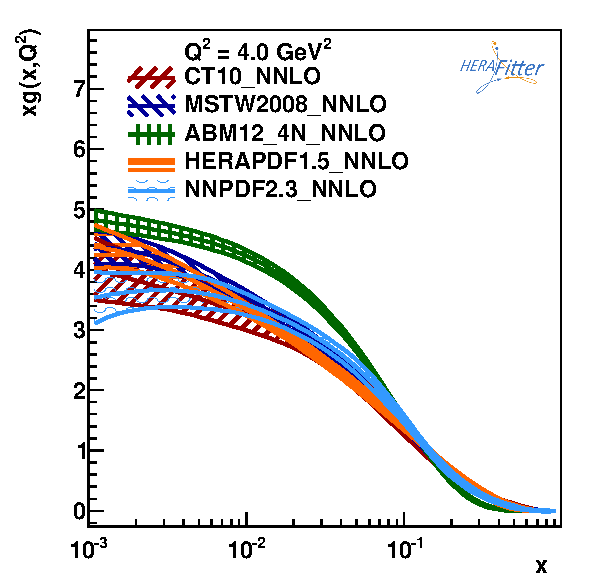
\includegraphics[width=8cm]{pdfs.pdf}
   \caption{Gluon density as extracted by various PDF groups at the scale of $Q^2=2$ GeV$^2$, plotted using the drawing tools from \fitter.} 
 \label{fig:pdfs}
\end{figure}
%
\subsection{Chisquare representation}
\label{sec:chi2representation}

The PDF parameters are extracted from a $\chi^2$ minimization process. 
There are various forms to represent the $\chi^2$ function, e.g. using a covariance matrix or decomposed into nuisance parameters. In addition, there are various methods to dealing with the correlated systematic (or statistical) uncertainties. Here we summarise the options available in \fitter\ . 

\begin{description}
\item \bf {Covariance Matrix Representation:} \rm
For a data point  $\mu_i$ with a corresponding theory prediction $m_i$, the $\chi^2$ function for the case when experimental uncertainties are given as a covariance matrix over data bins $C_{i,j}$ can be expressed in the following form:
%
\begin{eqnarray}
\chi^2 (m)& = & \sum_{i,j}(m_i-\mu_i)C^{-1}_{ij}(m_j-\mu_j).
\end{eqnarray}
%The $\chi^2$ function depends on the theory parameters $m^i$ 
%(denoted as the vector $\boldsymbol{m}$).
The covariance matrix can be decomposed in statistical, uncorrelated and correlated systematic contributions: 
\begin{eqnarray}
C_{ij}& = & C^{stat}_{ij}+C^{uncor}_{ij}+C^{sys}_{ij}.
\end{eqnarray}
This representation can not single out the effect of a particular
source of systematic.

\item \bf{Nuisance Parameters Representation:} \rm
\begin{eqnarray} 
    \chi^2\left(\boldsymbol{m},\boldsymbol{b}\right) &= &  
 \sum_i \frac{\left[m^i - \sum_j \gamma^i_j m^i b_j  - {\mu^i} \right]^2}
{ \textstyle \delta^2_{i,{\rm stat}}\mu^i \left(m^i -  \sum_j \gamma^i_j m^i b_j\right)
  + \left(\delta_{i,{\rm uncor}}\,  m^i\right)^2} \nonumber \\
  &+& \sum_j b^2_j.
\label{eq:aven}
\end{eqnarray}
%
Here ${\mu^i}$ is the  measured central value  at a point $i$ 
with  relative statistical $\delta_{i,stat}$ 
and relative uncorrelated systematic uncertainty $\delta_{i,unc}$.
Further, 
%$\beta_j$ denotes a nuisance parameter for
% a correlated systematic error  source of type $j$ with an uncertainty while
$\gamma^i_j$ 
quantifies the sensitivity of the
measurement ${\mu^i}$ at the point $i$ to the correlated systematic 
source $j$. The function $\chi^2$ depends in addition on
 the set of systematic nuisance parameters $b_j$.
This definition of the $\chi^2$ function assumes that
systematic uncertainties are proportional to the central prediction values
(multiplicative errors), whereas the statistical errors scale 
with the square root of the expected number of events. 
\item  \bf{Mixed Form:} \rm
It can happen that various parts of the systematic and statistical uncertainties are stored in different forms. A situation can be envisaged when the correlated systematic experimental uncertainties are provided as nuisance parameters, but the statistical bin-to-bin correlations are given in the form of a covariance matrix. \fitter\ offers the possibility to include such information, when provided, as well as any other mixed form of treating statistical, uncorrelated and correlated systematic uncertainties. 
%In the case of off-diagonal statistical uncertainties, the $\chi^2$ function
%\begin{equation} 
%\begin{eqnarray} 
% \label{eq:chi2gen}
%    \chi^2(\boldsymbol{m},\boldsymbol{b})& = & \sum_{ij} 
%         \left ( m^i - \sum_l \gamma^i_l(m^i)b_l - \mu^i \right)  C^{-1}_{{\rm stat.}~ij}(m^i,m^j) \nonumber \\  
%    && \left(  m^j - \sum_l \gamma^j_l(m^j)b_l - \mu^j \right) +  \sum_l b^2_l.
%\end{eqnarray}
%\end{equation}
%Here the scaling properties of the correlated systematic uncertainties 
%$\Gamma^i_j$ and
%of the covariance matrix $C_{{\rm stat.}~ij}$ are expressed as a dependence
%on $m_i$ and the dependence of $\delta_{\rm stat}$ on $b_j$ is ignored.
\end{description}


\subsection{Treatment of the Experimental Uncertainties}

\fitter\ provides three methods for assessing the experimental uncertainties on PDFs: the Hessian, Offset, and Monte Carlo methods, which are described below.
Figure \ref{fig:error} illustrates the difference between the Hessian and Monte-Carlo methods both of which can be applied and plotted with \fitter.
\begin{figure}[!ht]
   \centering
   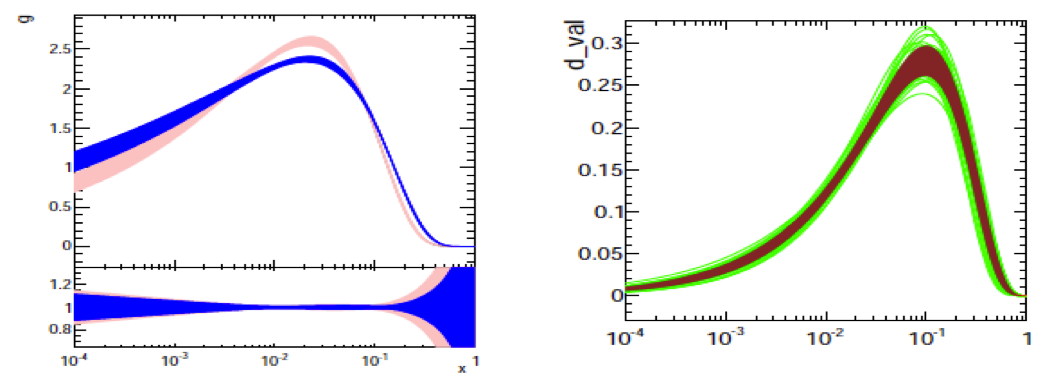
\includegraphics[width=8cm]{error.pdf}
   \put (-206, 68) {Hessian}
   \put (-86, 68) {Monte Carlo}
   \caption{Differences in the experimental uncertainties on the gluon (left) and d-valence quark (right) densities extracted 
       through different methods in \fitter: Hessian(left) versus Monte Carlo (right).} 
 \label{fig:error}
\end{figure}
\begin{description}
\item \bf{Hessian method:} \rm
The technique developed by \cite{Pumplin:2001ct} presents an estimate of PDF uncertainties reflecting the experimental precision of data used in the QCD fit by examining the behaviour of $\chi^2$ in the neighborhood of the minimum. The systmatic shift nuisance parameters $b_j$ as well as the PDF parameters are free parameters of the fit. Thus the fit determines the best fit to the data taking into account correlated systematic shifts of the data. This is known as Hessian or error matrix method. The Hessian matrix is build by the second derivatives of $\chi^2$ at the minimum. The PDF eigenvectors are obtained through an iterative procedure used to diagonalise the Hessian matrix and rescale the eigenvectors to adapt the step sizes to their natural scale.

\item \bf{Offset  method:} \rm

There is another method to propagate the correlated systematic experimental uncertainties from the measurements to PDFs \cite{Botje:2001fx}, which has the practical advantage that does not require the inversion of a large measurement covariance matrix.
%
It uses also the $\chi^2$ function for the central fit for which only
uncorrelated uncertainties are taken into account to get the best PDF parameters. The goodness of fit can no longer be judged from the $\chi^2$ since correlated uncertainties are ignored. 
%
The correlated systematic uncertainties of the data are then used to estimate 
the errors on the PDF parameters as follows.
Taking each systematic source in turn the value of the cross section is offset 
by its one sigma shift from the central value and the fit is performed again.
This is done for both psotive and negative one sigma shifts. 
After this has been done for all sources the 
resulting deviations of each of these fits from the central PDF parameters are added in quadrature. 

In most cases, the uncertainties estimated through offset method are larger than those from the Hessian method, as the offset method does not use the information on correlated systematic uncertainties optimally.

\item \bf{Monte Carlo method:} \rm
The PDF uncertainties can be estimated using a Monte Carlo technique \cite{Giele:1998gw, mcmethod2}.
The method consists in preparing replicas of data sets by allowing the central values of the cross sections to 
fluctuate within their systematic and statistical uncertainties taking into account all point-to-point correlations.
The preparation of the data is repeated for a large $N$ ($>100$ times) and for each of these replicas a NLO QCD fit is performed to 
extract the PDF set. The PDF central values and uncertainties are estimated using the mean values and RMS 
over the replicas. 
\end{description}


\subsection{Treatment of the Theoretical Input Parameters}

The results of a QCD fit depends not only on the input data but also on the 
input theoretical ansatz, which is also uncertain. Nowadays, modern PDFs 
try to address the impact of the choices of theoretical parameters by providing
alternative PDFs with different choices of the mass of charm $m_c$, mass of the bottom quarks $m_b$ and the value of $\alpha_S(M_Z)$, etc. 
Another important input is the choice of the functional form for the PDFs at the starting scale and indeed the value of the starting scale itself. \fitter\ provides a platform in which such choices can readily be varied within a common framework.


\subsection{Performance Optimisation}

The above mentioned features make \fitter a powerful project that encapsulates 
state of the art developments from the most up-to-date theory developments to
debates on reacing the ultimate experimental precision. 

An important factor for a feasible QCD fit which is performed by iterative 
$\chi^2$ minimisation, is performance in terms of how long a calculation takes for each given data point.
The performance of the \fitter  code is greatly improved with several special built-in options
including the $k-factor$ techniques (described in section~\ref{sec:techniques}), the grid techniques for the fast calculation of cross 
sections of particular processes for arbitrary sets of PDFs (section~\ref{sec:techniques}). There are also cache options, fast evolution kernels, and 
usage of the openMP (Open Multi-Processing) interface which allows
parallel applications of some of the heavy flavour scheme theory predictions in DIS. {\bf please go over this, I have married two separate paragraphs that were in different places}

{\bf You mentioned reeighting techiniques, but in fact they have NOT been described in this section}





